\documentclass{article}


\usepackage[T1]{fontenc}
\usepackage[czech]{babel}
\usepackage[utf8]{inputenc}
\usepackage{graphicx}
\usepackage{biblatex}
\usepackage{mathtools}
\usepackage{hyperref}

\usepackage{listings}
\usepackage{xcolor}
\lstdefinelanguage{JavaScript}{
  keywords={typeof, new, true, false, catch, function, return, null, catch, switch, var, if, in, while, do, else, case, break},
  keywordstyle=\color{blue}\bfseries,
  ndkeywords={class, export, boolean, throw, implements, import, this},
  ndkeywordstyle=\color{darkgray}\bfseries,
  identifierstyle=\color{black},
  sensitive=false,
  comment=[l]{//},
  morecomment=[s]{/*}{*/},
  commentstyle=\color{purple}\ttfamily,
  stringstyle=\color{red}\ttfamily,
  morestring=[b]',
  morestring=[b]"
}

\lstset { %
    language=JavaScript,
    backgroundcolor=\color{black!5}, % set backgroundcolor
    basicstyle=\footnotesize,% basic font setting
}

\graphicspath{ {imgs/} }
\def\code#1{\texttt{#1}}	

\title{NPRG045 Ročníkový projekt (Individual project)}
\author{Štěpán Klos}
\date{}

\begin{document}
\maketitle

In this document we will guide reader through the process of setting up custom Kubernetes cluster. We will show it's specific features to facilitate process of deploying and running web applications in it.
\bigbreak
Kubernetes is an open-source container orchestration tool bringing new modern approach for running web applications in the cloud. Kubernetes was created by Google in 2014 and written in Go. Running production on open-source software, however, comes without any guarantees. Thus, a market for commecrial products arised. In this document we will not only present the setup per-se but also compare managed providers with self-hosted commercial solutions to self-hosted plain Kubernetes. \par
\bigbreak
We will break down each step of the process ranging from overview to actual deployment on specific cloud provider.   

\section{Problem description}
There are several motivations that led to the creation of Kubernetes. Environment isolation and scaling are the most significant ones. We want to have an "universal runtime environment" of various technologies to satisfy needs of developers and necesities of our company. These might range from developers needing various versions of PHP and different installed libraries to robust .NET backend, Remote Dictionary Server for session sharing, different frontends with client-side routing defined by developer (with no need of editing webserver or breaching rules for htaccess) or even microservices. 
\subsection{Stack mismatch across projects}
We can encouter different needs within organization. Oldschool approach to having servers with usually one runtime fails since each user can have slightly different needs.
\subsubsection{Backend tech and library needs}
We have more (not necessarily) PHP backend projects. We need isolation to accomodate different backend technologies and version. There even might a be demand for different versions of one specific library.
\begin{itemize}
  \item Applications running PHP 5.6.0 (ft. MySQL).
  \item Applications running PHP 8.0.0 (ft. MySQL).
  \item Application running PHP 7.2.24 + imagecreate + ZipArchive (ft. MySQL).
  \item Applications running Node.js + custom stuff from package.json.
\end{itemize}
\subsubsection{Frontend configuration stuff}
Configuration might be tricky for different reason. \textbf{Firstly}, we need to have \textbf{rewrites} allowed.
\begin{lstlisting}
  a2enmod rewrite
  systemctl restart apache2
\end{lstlisting}
\textbf{Secondly}, client-side routing settings of the webserver might not be overridable via \textbf{.htaccess}.  
\begin{lstlisting}
  Options +FollowSymLinks
  Options -MultiViews
  RewriteEngine On
  RewriteCond %{REQUEST_FILENAME} !-f
  RewriteCond %{REQUEST_URI} !^/route-exception/
  RewriteRule ^ index.html [QSA,L]
\end{lstlisting}
The settings has to be done on root of Apache which is a request (and potential security breach) on the administrator.
\begin{lstlisting}
  # :443 for https
  <VirtualHost *:80>
    DocumentRoot /var/www/html
    <Directory /var/www/html/>
        AllowOverride All
        Options FollowSymLinks
    </Directory>
    <IfModule mod_security2.c>
        SecRuleEngine DirectionOnly
    </IfModule>
  </VirtualHost>	
\end{lstlisting}
\subsection{Scaling}
Hosting several applications on one server or one by one might bring scaling problems. Kubernetes allows interfacing with cluster...which has independent attachagle worker nodes. workloads can then automatically scale making great for variable production (Cluster IMG + M+Ws IMG)
\begin{lstlisting}

\end{lstlisting}
\subsection{Different images preparation}
mby
\subsection{Virtual infrastructure objects - redo, in next chapter}
- routing
- applications running
- different runtimes PHP / libs
- difrerent libraries
- izolation / scaling
\section{Virtualization w/ Kubernetes}
\subsection{cgroups}
Control groups \textbf{cgroups} play a major role in isolation of running processes within Linux kernel.  

\subsection{Image structure}
Images are layered... built...etc.
\begin{center}
  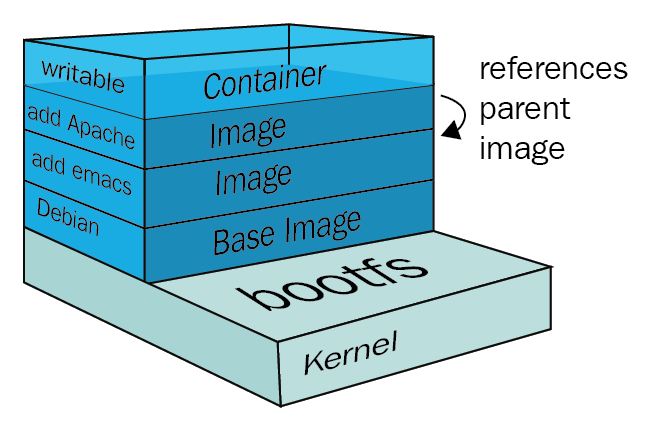
\includegraphics[width=0.450\textwidth]{000_Image_structure.png}
\end{center}
\subsection{Open Container Initiative}
The Open Container Initiative is an open governance structure for the express purpose of creating open industry standards around container formats and runtimes.
\subsection{History}
mby some history
\subsection{Breakdown of Kubernetes objects}
Kubernetes clusters have similar architecture regardless of provider or author. Despite some differences, the main core objects and flows are the same. We will  
\subsubsection*{Cluster Architecture}
Cluster architecture refers to the arrangement and organization of nodes within a Kubernetes cluster. In a Kubernetes cluster, there are different types of nodes, including the master node and worker nodes. The master node manages the overall cluster, while the worker nodes execute the tasks and run the containers. The Kubernetes API is a core component that allows communication and interaction with the cluster, enabling users to control and manage the cluster's resources and workloads.

Nodes - Master Node, Worker Nodes, (The Kubernetes API)
\subsubsection*{Workload}
Workload in Kubernetes refers to the tasks or applications that run within the cluster. Kubernetes provides several resources to define and manage workloads effectively. Deployments are used to define and manage pods, which are the basic units of execution in Kubernetes. ReplicaSets, controlled by deployments, ensure the desired number of pod replicas are running. These resources enable easy scaling, rolling updates, and self-healing for applications running in the cluster.


Deployments - define Pods and ReplicaSets
\subsubsection*{Services, Load Balancing, and Networking}
Services in Kubernetes provide a stable network endpoint to access a set of pods. They act as an abstraction layer, enabling load balancing across multiple pods and allowing seamless communication between them. Services have a specific port through which they can be accessed and a targetPort that defines the port where the pods receive traffic. Load balancing ensures that the traffic is distributed evenly among the available pods. Ingress is another resource that provides external access to services within the cluster, allowing for routing and other advanced networking capabilities.

Ingress
Service (port, targetPort)
\subsubsection*{Storage}
Storage in Kubernetes is managed through various resources. Volumes provide a way to store data within a pod and are often used for temporary or short-lived data. Persistent Volumes (PVs) are a more long-term storage solution, decoupled from pods, and can be dynamically provisioned or pre-allocated. Persistent Volume Claims (PVCs) are used by applications to request specific storage resources from PVs, allowing for flexibility and scalability in storage management.


Volume - Persistent Volume
Persistent Volume Claim
\subsubsection*{Configuration}
In Kubernetes, configuration management involves handling sensitive information and application settings. Secrets are resources used to store and manage sensitive data, such as passwords, API keys, or TLS certificates. They are encrypted and can be securely accessed by pods. Secrets are commonly used to provide secure access to external services or to configure applications with sensitive information.

Secret
\subsubsection{Tasks}
HorizontalPodAutoscaler (HPA) is a resource in Kubernetes that automates the scaling of deployments based on CPU utilization or custom metrics. It dynamically adjusts the number of replicas for a deployment to ensure efficient resource utilization and accommodate changes in workload demand. By automatically scaling up or down, the HPA helps maintain optimal performance and responsiveness of applications running in the cluster. The HPA is typically attached to a deployment, allowing it to monitor and control the scaling behavior for that specific workload.

HorizontalPodAutoscaler - attached to Deployment

Setup Load balancer, Ingress, Aplikace, Servisy
\section{Technical setup}
Our technical setup on DigitalOcean (based on prev. general setup) \par
Technical setup of components
Viz. repo but cloud agnostic
Setup, nodes, services
\section{Environment comparison}
\subsection{Self hosted vs. Managed}
Self hosted - Master, Worker (attaching), machines/VPS
Managed - Just service
\subsection{Minikube}
Minikube - all-in-one

- self hosted options(Open Shift, Tanzu, plain Kubernetes) vs. managed options (AWS/Azure AKS/DigitalOcean Kubernetes)
- services by provider vs self-hosted within cluster (within cloud provirers)
Comparison admin screenshots, + and -s, table comparison
Implementation on DigitalOcean https://github.com/KlosStepan/DOKS-tutorial
\section{Application deployments}
Combination of Ingress with services, deployments
\subsection{Deployment of Redis}
\subsection{Deployment of MySQL into Cluster}
PHP app, React app, CI/CD pipelines
\section{Cluster Administration}
\subsection{kubectl}
\subsection{Kubernetes Dashboard}
\subsection{Lens}
\subsection{CI/CD Pipelines}
Worflows and Azure Pipelines
\section{Outtro}
We succeded after several tryouts and self-hosted stuff which we described.
SLA option (?)
\section{Tools and software}

We are using these parts and tools:
\begin{itemize}
\item Oracle 18.3 \footnote{https://docs.oracle.com/en/engineered-systems/oracle-database-appliance/18.3/index.html} on server,
\item ORACLE SQL Developer 21.4.3 \footnote{https://www.oracle.com/database/sqldeveloper/technologies/21.4.3-release-notes/},
\item node-oracledb 5.3.0 \footnote{https://www.npmjs.com/package/oracledb/v/5.3.0},
\item features facilitating the development and working.
\end{itemize}

\newpage

\section{Initial steps and setup}
So we prepare ourselves by unzipping the newest version of \textbf{sqldeveloper} in our computer. Then we open it and right click \textbf{Import Connections} select encrypted json file with connector to our database provided by our collegues or us (if we created the database previously).  \par
\begin{center}
\includegraphics[width=0.250\textwidth]{01_Import_crop.png}
\end{center}
We navigate the \textbf{import connection} manager and fill out optional password to the connection file (if needed). By following this form we will have created created authorized Oracle Connections to our database(s). \par
\begin{center}
  \includegraphics[width=0.450\textwidth]{02_Import_crop.png}
\end{center}
Once we are ready, we see that solution automatically comes with \textbf{production database} and \textbf{test database}. We will be working strictly on the test database until we're ready to ship tested aplication to production. After loading we can see various database related things on the left side, most importantly \textbf{Tables}, \textbf{Views}, \textbf{Procedures}, \textbf{Functions} and other stuff. We will go through these items and show some Oracle features such as BLOBs and native inserts/selects with json\_object for "ORM-like" interfacing with database. \par
\begin{center}
  \includegraphics[width=0.850\textwidth]{03_Database.png}
\end{center}

\section{Interfacing with Oracle Database from Node.js}
Oracle Database will be used for a web application. We need to connect to our database with Node.js as client language for backend. There are several things which are different from "typical PHP-MySQL connection" which is (former) de facto status quo in web development. To deliver REST API we need to: 
\begin{itemize}
\item install \textbf{oracledb} package via npm\footnote{Run "npm install oracledb" for https://www.npmjs.com/package/oracledb},
\item serialize listings in database for backend,
\item send desired responses via HTTP REST endpoints.
\end{itemize}
After we install oracledb, we need to connect to database. For such task, we create object with \textbf{username}, \textbf{password} and a \textbf{connector line} which is not going to be in GIT repo for security reasons. We include use this object as an argument for connection. \par
\textbf{\_dbCreds.js}
\begin{lstlisting}
  module.exports = {
    user: 'user',
    password: 'passwd',
    connectString: "(DESCRIPTION=(ADDRESS_LIST=(FAILOVER=true)
    (LOAD_BALANCE=false)(ADDRESS=(PROTOCOL=TCP)(HOST=HHHH)
    (PORT=PPPP))(ADDRESS=(PROTOCOL=TCP)(HOST=HHHH)
    (PORT=PPPP)))(CONNECT_DATA=(SERVICE_NAME=SSSS)))"
  }
\end{lstlisting}  
\textbf{dbConn.js}
\begin{lstlisting}
const oracledb = require('oracledb');
const dbCreds = require("./_dbCreds");
let database = null;
async function startDatabase() {
  database = await oracledb.getConnection(dbCreds)
}
async function getDatabase() {
  if (!database) await startDatabase();
  return database;
}
module.exports = {
  getDatabase,
  startDatabase
};
\end{lstlisting}
Noteworthy item here is the connectionString \footnote{For more information https://docs.oracle.com/database/121/ODPNT/featConnecting.htm\#ODPNT166} which must be included to specify connection creds. Then we can execute queries thanks to classes as follows:
\begin{lstlisting}
const { getDatabase } = require("./dbConn");
async function f() {
  let connection = await getDatabase();
  let query = "select ... from view"
  result = await connection.execute(query);
}
\end{lstlisting}
\section{Construction of REST API}
We will outline several types of endpoints which are needed not only in our applicaton but in general. Some of ours, however, utilise serialization of SELECT via json\_object in Oracle Database, some send picture from assembled bytestream from database BLOB, some server for insertions, etc.
\subsection{Listing REST endpoint - GET / }
Most straightforward is endpoint providing listing of elements. These endpoints return \textbf{View} (with joined lists from other table affiliated) and returns entries as JSON thanks to json\_object \footnote{More about json\_object https://docs.oracle.com/en/database/oracle/oracle-database/12.2/sqlrf/JSON\_OBJECT.html\#GUID-1EF347AE-7FDA-4B41-AFE0-DD5A49E8B370}. \textbf{select * from v\_listingvybaveni}
\begin{lstlisting}
  CREATE OR REPLACE FORCE EDITIONABLE VIEW "APP_KDP_V1"
  ."V_LISTINGVYBAVENI" ("JSRECORD") AS
  with vp as (
    select
        vybaveni_id
        , '[' || listagg('{"rodina_kod":"' || rodina_kod
         || '", "pouzitiId":' || pouziti_id || '}',', ')
          WITHIN GROUP (ORDER BY rodina_kod) || ']' vybaveniPouziti
    from vybaveni_pouziti
    group by vybaveni_id
),
f as(
    select
        prvek_id
        , '[' || listagg('{"fotoId":'|| id ||'}',', ')
          WITHIN GROUP (ORDER BY poradi) || ']' foto
    from foto
    group by prvek_id  
)
select json_object(
        'id' value v.id,
        'kod' value v.kod,
        'design' value v.design,
        'nazev' value v.nazev,
        'popis' value v.popis,
        'ergonomie' value v.ergonomie,
        'material' value v.material,
        'servis' value v.servis,
        'certifikat' value v.certifikat,
        'modifikace' value v.modifikace,
        'dostupnost' value v.dostupnost,
        'cenovahladina' value v.cenovahladina,
        'viditelnost' value v.viditelnost,
        'vybaveniPouziti' value vp.vybaveniPouziti format json,
        'foto' value f.foto format json
    )
from vybaveni v
left join vp on vp.vybaveni_id = v.id
left join f on f.prvek_id = v.id;
\end{lstlisting}
\subsection{Image backend service via BLOB - GET /id}
We store images in database in BLOBs and have endpoint which will deliver upon request. This is the function to retrieve and return BLOB \footnote{https://docs.oracle.com/database/121/TDPPH/ch\_twelve\_blobs.htm\#TDPPH183}.
\begin{lstlisting}
//Foto for BE function
async function retrieveFotoById(req, res, fotoId) {
  let connection;
  try {
    connection = await getDatabase();
    const result = await connection
    .execute("SELECT image FROM FOTO WHERE id='"+fotoId+"'");
    if (result.rows.length === 0) {
      throw new Error("No data selected from table.");
    }
    const lob = result.rows[0][0];
    if (lob === null) {
      throw new Error("BLOB was NULL");
    }
    const doStream = new Promise((resolve, reject) => {
      lob.on('end', () => {
        res.end();
      });
      lob.on('close', () => {
        resolve();
      });
      lob.on('error', (err) => {
        reject(err);
      });
      res.writeHead(200, {'Content-Type': 'image/jpeg' });
      lob.pipe(res);  // write the image out
    });
    await doStream;
    connection = null;
  } catch (err) {
    console.error(err);
    await closePoolAndExit();
    } finally {
    if (connection) {
      try {
        await connection.close();
      } catch (err) {
      console.error(err);
      }
    }
  }
}
async function closePoolAndExit() {
  try {
    await oracledb.getPool().close(2);
    process.exit(0);
  } catch (err) {
    console.error(err.message);
    process.exit(1);
  }
}
\end{lstlisting}
Selected image get streamed with header to client via backend as a HTTP response. Preview of parametrized query is possible to be viewed in SQL Developer even with "image representation of bytestream" - which in this case is a JPEG image. \par
\includegraphics[width=0.990\textwidth]{05_BLOB.png}
Application endpoint for image, therefore, returns an image, which in reality doesn't even have to occupy a space as a file on server's filesystem, which for dummy previews like these is very elegant way of simplifying application. \par
\bigbreak
Requests, thus can arrive as responses from \textbf{kdp.ipr.praha.eu/api/foto/154} and can be placed into HTML img source tag directly. Backend side of things is as straightforward as one would expect. Function \textbf{retrieveFotoById(params)} was described above for sending HTTP headers and streaming picture's bytestream. \par
\bigbreak
\textbf{index.js} of Node.js express backend, with app being instance of Express \footnote{https://expressjs.com} running on sbds.domain.tld\textbf{/api}
\begin{lstlisting}
app.get('/foto/:fotoId', async(req, res) => {
  res.send( await retrieveFotoById(req, res, req.params.fotoId))
})  
\end{lstlisting}
\textbf{DisplayFoto.jsx} function component on React.js \footnote{https://reactjs.org} frontend 
\begin{lstlisting}
import URLEndPointBE from './URLEndPointBE'
function DisplayFoto(props) {
  const fotoEndpoint = URLEndPointBE + `/foto`
  return(
    <span><img src={fotoEndpoint+"/"+props.foto.fotoId}</span>
  )
}
export default DisplayFoto
\end{lstlisting}
\section{Oracle SQL Developer description}
Going back to Oracle SQL Developer, there are some noteworthy things that have to be said about features and functions. These features facilitate process of working on database or viewing the data or even fiddling with it. 
\subsection*{Worksheet section} 
 After opening Oracle SQL Developer and connecting to one database, a \textbf{Welcome page} pops up. It is notebook-worksheety tool, to execute SQL queries that are not necessarily affiliated to any specific part. One can, however, run queries or SQL statements to create functions or preform whatever actions that do (not) modify database structure/content. \par
 \bigbreak
 Looking up, you can either \textbf{Run Statement (Ctrl+Enter)} or \textbf{Run Script (F5)} which differ in the readability of output, run statement returns  aw data but run script returns you more verbous human-readable output. \par
\bigbreak
\includegraphics[width=0.990\textwidth]{06_Worksheet.png}
\newpage
\subsection*{Table Model} 
Visualized realtions of selected table with other tables. \par
\includegraphics[width=0.990\textwidth]{07_TableModel.png}
\subsection*{Views SQL code example}
Views editation preview in Oracle SQL Developer - img here, selection query as well. \par
\includegraphics[width=0.990\textwidth]{08_ViewSQL.png}

\end{document}
